\documentclass{article}
\usepackage{graphicx}
\usepackage{amsmath}
\graphicspath{ {./figures/} }

\title{TP MATLAB : Transformée de Fourier}
\date{9 Janvier 2021}
\author{Lucas LOISEAU \\ Alexandre SENOUCI \\ Maya BROYER \\ Lena BELIAZI}

\begin{document}
\maketitle
\section{Transformée de Fourier discrète}
Les signaux sont représentés sur l'intervalle $[-5,5]$. \\
On fixe le nombre d'échantillons à $N=32768$. \\
La période d'échantillonage vaut donc $T_e = 3,0518 * 10^{-4}$ et la fréquence d'échantillonage $f_e=3276,8$.11111
\subsection{Echantillonage et spectre de fonctions usuelles}
\subsubsection{Fonction constante}
On considère la fonction $x_0(t)=42$ dont la transformée de Fourier théorique est $X_0(f)=\delta(f)$, il s'agit d'un nombre réel donc nous affichons uniquement la partie réelle de la transformée de Fourier calculée numériquement.
\begin{figure}[h]
\includegraphics[scale=0.5]{fig_const}
\centering
\end{figure}
\subsubsection{Fonction cosinus}
On considère la fonction $x_1(t)=\cos(2\pi f_0 t)$ avec $f_0=4$, sa transformée de Fourier théorique est $X_1(f)=\frac{1}{2}[\delta(f-f_0)+\delta(f+f_0)]$, il s'agit d'un nombre réel.

\begin{figure}[h]
\includegraphics[scale=0.63]{fig_cos}
\centering
\end{figure}

\subsubsection{Fonction sinus}
On considère la fonction $x_2=\sin(2\pi f_0 t)$ avec $f_0=4$, sa transformée de Fourier théorique est $X_2(f)=\frac{1}{2j}[\delta(f-f_0)-\delta(f+f_0)]$, il s'agit d'un imaginaire pur.
\begin{figure}[h]
\includegraphics[scale=0.6]{fig_sin}
\centering
\end{figure}

\subsubsection{Fonction pic de Dirac}
On considère la fonction $x_3(t)=\delta(t-\Delta t)$, sa transformée de Fourier théorique est $X_3(f)=e^{-j2\pi f\Delta t}$. \\
Lorsque $\Delta t$ est nul, nous constatons bien que la transformée de Fourier du Dirac est constante à $1$ :
\begin{figure}[h]
\includegraphics[scale=0.6]{fig_dirac_0}
\centering
\end{figure} \\
Tandis qu'avec un décalage temporel $\Delta t$ non nul, nous obtenons les courbes suivantes :
\begin{figure}[h]
\includegraphics[scale=0.6]{fig_dirac_deltat}
\centering
\end{figure} \\
Ce qui correspond bien à $Re(X_3(f))=\cos(2\pi f\Delta t)$ et $Im(X_3(f))=\sin(2\pi f\Delta t)$

\subsubsection{Exponentielle complexe}
On considère la fonction $x_4=e^{j2\pi f_0 t}$ qui a comme transformée de Fourier théorique $X_4=\delta(f-f_0)$.
\begin{figure}[h]
\includegraphics[scale=0.6]{fig_exp}
\centering
\end{figure} \\
La transformée de Fourier donne bien $\delta(f-f_0)$ (avec $f_0=4$ sur cette figure).

\subsubsection{Foncion rectangle}
\paragraph{Fonction rectangle apériodique}
Nous allons analyser la fonction rectangle dont la transformée de Fourier théorique est un sinus cardinal.
\begin{figure}[h]
\includegraphics[scale=0.6]{fig_rect}
\centering
\end{figure}
\paragraph{Fonction rectangle périodique}
Nous considérons cette fois une fonction rectangle rendue périodique.
\begin{figure}[h]
\includegraphics[scale=0.6]{fig_rect_per}
\centering
\end{figure} \\
La transformée de Fourier donne cette fois un sinus cardinal discrétisé.
\subsubsection{Courbe de Gauss}
La dernière fonction que nous allons analyser est une courbe de Gauss dont l'équation est $x_6(t)=\exp(-\pi t^2)$
\paragraph{Calcul de la transformée de Fourier théorique}
$$X_6(f) = \int_{-\infty}^{\infty}e^{-\pi t^2}e^{-j2\pi ft}dt=\int_{-\infty}^{\infty}e^{-(\pi t^2 +j2\pi ft)}dt$$. \\
On pose alors
$$\left\{\begin{array}{l}
a^2=\pi t^2 \\
2ab = j2\pi ft
\end{array}\right.
\Rightarrow
\left\{
\begin{array}{l}
a^2=\pi t^2 \\
b^2=-\pi f^2
\end{array}
\right.
$$
L'intégrale se réécrit
$$\int_{-\infty}^{\infty}e^{-(a^2+2ab+b^2)+b^2}dt=\int_{-\infty}^{\infty}e^{-(a+b)^2+b^2}dt$$
On effectue le changement de variable $X=a+b=\pm(\sqrt{\pi}t + j\sqrt{\pi}f)$ avec $\frac{dX}{dt}=\pm \sqrt{\pi}\Leftrightarrow dt=\frac{dX}{\pm\sqrt{\pi}}$ \\
Ce qui donne
$$\int_{-\infty}^{\infty}e^{-X^2-\pi f^2}\frac{dX}{\pm\sqrt{\pi}}=\frac{1}{\pm\sqrt{\pi}}e^{-\pi f^2}\int_{-\infty}^{\infty}e^{-X^2}dX=\pm e^{-\pi f^2}$$
En admettant que $\int_{-\infty}^{\infty}e^{-x^2}dx=\sqrt{\pi}$
\paragraph{Calcul de la transformée de Fourier avec MATLAB}
Nous obtenons le spectre suivant :
\begin{figure}[h]
\includegraphics[scale=0.52]{fig_gauss}
\centering
\end{figure}
\section{Echantillonage et repliement de spectre}
On se propose d'étudier la famille de fonctions paramétriques 
$$g_f(t)=\sin(2\pi f t)+\sin(2\pi(f+\Delta f)t)+\sin(2\pi(f+2\Delta f)t)+2\sin(2\pi(f+3\Delta f)t)$$

avec $\Delta f=50$
\subsection{Calcul des spectres théoriques de $g_{1000}$ et $g_{2250}$}
En exploitant la linéarité de la transformée de Fourier ainsi que le résultat $\sin(2\pi f_0 t)=\frac{1}{2j}[\delta(f-f_0)-\delta(f+f_0)]$, nous obtenons : \\
$$G_{1000}=\frac{1}{2j}[\delta(f-1000)-\delta(f+1000)+\delta(f-1050)-\delta(f+1050)+\delta(f-1100)-\delta(f+1100)+2\delta(f-1150)-2\delta(f+1150)]$$
$$G_{2250}=\frac{1}{2j}[\delta(f-2250)-\delta(f+2250)+\delta(f-2300)-\delta(f+2300)+\delta(f-2350)-\delta(f+2350)+2\delta(f-2400)-2\delta(f+2400)]$$
\newpage
\subsection{Spectres avec échantillonage}
Pour la fonction $g_{1000}$, nous obtenons le spectre suivant :
\begin{figure}[h]
\includegraphics[scale=0.5]{fig_g1}
\centering
\end{figure} \\
Cela correspond à nos attentes, nous retrouvons bien des pics de fréquence aux valeurs $\pm1000$, $\pm1050$, $\pm1100$ et $\pm1150$.
En revanche, pour la fonction $g_{2250}$, les pics de fréquences obtenus sont incorrects :
\begin{figure}[h]
\includegraphics[scale=0.5]{fig_g2}
\centering
\end{figure} \\
Cela s'explique par le fait que la fréquence maximale du signal $f_{max}=2400\,\mathrm{Hz}$ soit supérieure à la moitié de la fréquence d'échantillonage $f_e=3276,8 \,\mathrm{Hz}$. Un phénomène de repliement de spectre se produit alors et cause l'apparition de fréquences parasites dans le signal.
\section{Transmission par modulation d'amplitude}
\subsection{Opération de modulation sur deux signaux}
\subsubsection{Signaux étudiés}
Nous allons moduler les deux signaux suivants :
$$ s_1(t) = \sum_{n=1}^{10}n\cos(2\pi.10n.t)$$
\begin{figure}[h]
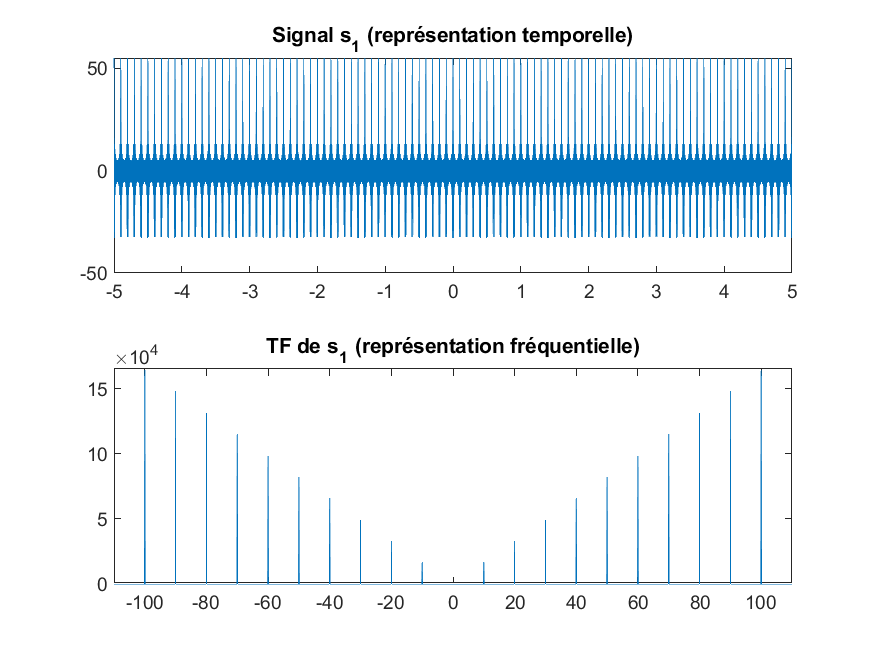
\includegraphics[scale=0.5]{fig_s1}
\centering
\end{figure}
$$ s_2(t)=\sum_{n=1}^{10}(11-n)\cos(2\pi.10n.t)$$
\begin{figure}[h]
\includegraphics[scale=0.5]{fig_s2}
\centering
\end{figure}
\subsubsection{Opération de modulation}
Nous allons maintenant calculer le signal modulé $m(t)$ ayant la propriété de contenir tous les signaux $s_i(t)$. Voici son expression :
$$m(t)=\sum_{i}s_i(t).\cos(2\pi f_i t)$$
Les fréquences $f_i$ propres à chaque signal $s_i(t)$ sont appelées fréquences porteuses.
\section{Filtrages}
\section{Localisation de formes par Corrélation}
\end{document}